%======================================================================
\chapter{Results and Discussion}
\label{ch:results}

This chapter reports the measured results of every station, compares them with the Phase 1 approach and with the targets set in Chapter~\ref{ch:intro}, and discusses what they do and do not show. Unless stated otherwise, accuracy figures are on held-out test splits that were not used for training, model selection, or threshold setting.

\section{Experimental Setup}
\label{sec:setup}
Training ran on an NVIDIA RTX A5000 (24\,GB). All latency figures were measured inside the production Docker image on one workstation (RTX A5000, Intel Xeon W-2295 with 36 threads, CUDA 12.1 PyTorch build 2.4.1, TensorRT 10.16.1, Ultralytics 8.4.192, ONNX Runtime 1.31.1 with the CPU provider). Each GPU configuration was warmed up with 5 calls and timed over 100 calls; medians are reported. Station 1 accuracy is reported for both the trained FP32 checkpoint and the deployed FP16 engine. Label-prototype results come from the experiments on the \texttt{himalaya-label-detection} branch and are reported with the protocol under which each number was obtained.

\section{Experimental Results}
\label{sec:experimental-results}

\subsection{Cap dataset and artefacts (O1)}
\label{sec:res-o1}
Table~\ref{tab:capdata} gives the per-class counts found on disk. The Roboflow export notes 8,530 images, but the three splits contain 8,524. Every image shows one bottle neck with one annotated cap, captured at $2048{\times}2048$ (a handful at $2048{\times}1536$) against indoor backgrounds. The training split holds 2,486 source photographs, each exported in three augmented versions (rotation $\pm5^\circ$, brightness $\pm25\%$, blur up to 2\,px, 0.5\% salt-and-pepper noise); validation and test images are not augmented. The masks come from a single annotator, so inter-annotator agreement cannot be measured.

\begin{table}[htbp]
\centering
\caption{Six-class cap dataset (one cap per image)}
\label{tab:capdata}
\footnotesize
\begin{tabular}{|l|r|r|r|r|}
\hline
\textbf{Class} & \textbf{Train} & \textbf{Valid} & \textbf{Test} & \textbf{Share of train} \\ \hline
good\_cap & 4,242 & 405 & 201 & 56.9\% \\ \hline
wet\_cap & 828 & 79 & 39 & 11.1\% \\ \hline
open\_cap & 768 & 65 & 38 & 10.3\% \\ \hline
damaged\_cap & 648 & 62 & 31 & 8.7\% \\ \hline
no\_cap & 645 & 61 & 30 & 8.6\% \\ \hline
misplaced\_cap & 327 & 40 & 15 & 4.4\% \\ \hline
\textbf{Total images} & \textbf{7,458} & \textbf{712} & \textbf{354} & \\ \hline
Source photographs & 2,486 & 712 & 354 & \\ \hline
\end{tabular}
\end{table}

The cap is not a small object in this dataset: its median bounding box covers 9.2\% of the test image (10th--90th percentile 6.0--14.0\%), and after resizing to the 640-pixel network input every instance is ``large'' by the COCO definition ($\geq96^2$ pixels)~\cite{lin2014coco}. What is small is the evidence inside the cap: droplets on wet caps, dents on damaged caps, and the thread gap of open caps. ``Small-object-aware'' in the primary objective therefore refers to preserving fine intra-object detail, which is what the distillation sites target, rather than detecting tiny objects.

Table~\ref{tab:artefacts} lists the exported artefacts of the cap model. The FP16 engine is about half the size of the FP32 ONNX graph, and Section~\ref{sec:res-seg} shows that it keeps the model's accuracy. As the benchmark for future model versions, a held-out test grouped by capture session has been identified, so that images of the same session never appear in both training and test.

\begin{table}[htbp]
\centering
\caption{Cap model artefacts}
\label{tab:artefacts}
\footnotesize
\begin{adjustbox}{max width=\textwidth}
\begin{tabular}{|l|l|r|l|}
\hline
\textbf{Artefact} & \textbf{Precision} & \textbf{Size (MB)} & \textbf{Use} \\ \hline
PyTorch checkpoint (\texttt{best.pt}) & FP32 & 45.2 & Training, PyTorch fallback \\ \hline
ONNX graph & FP32 & 90.5 & Portable runtime, TensorRT input \\ \hline
TensorRT engine (\texttt{best\_v1.engine}) & FP16, dynamic batch & 49.1 & Deployment on the target GPU \\ \hline
\end{tabular}
\end{adjustbox}
\end{table}

\subsection{Distillation outcome}
\label{sec:res-kd}
Table~\ref{tab:kd} compares teacher and student, both evaluated in FP32 with the same Ultralytics validation on the same splits. Figure~\ref{fig:curve} shows the student's validation mAP during distillation training.

\begin{table}[htbp]
\centering
\caption{Teacher versus distilled student (FP32, 640\,px)}
\label{tab:kd}
\footnotesize
\begin{tabular}{|l|c|c|}
\hline
 & \textbf{Teacher YOLO11x-seg} & \textbf{Student YOLO11m-seg} \\ \hline
Parameters (M) & 62.06 & 22.34 \\ \hline
GFLOPs @640 & 297.4 & 113.0 \\ \hline
Checkpoint size (MB) & 124.8 & 45.2 \\ \hline
Inference per image (ms)$^{*}$ & 19.0 & 7.8 \\ \hline
\multicolumn{3}{|l|}{\textit{Test split ($n=354$)}} \\ \hline
Box precision / recall & 0.995 / 0.997 & 0.998 / \textbf{1.000} \\ \hline
Box / mask mAP@0.5 & 0.995 / 0.995 & 0.995 / 0.995 \\ \hline
Box mAP@0.5:0.95 & \textbf{0.944} & 0.927 \\ \hline
Mask mAP@0.5:0.95 & 0.912 & \textbf{0.927} \\ \hline
\multicolumn{3}{|l|}{\textit{Per-class mask mAP@0.5:0.95 (test)}} \\ \hline
damaged / good & 0.929 / 0.877 & 0.927 / \textbf{0.893} \\ \hline
misplaced / no cap & 0.899 / 0.913 & \textbf{0.941} / 0.915 \\ \hline
open / wet & 0.931 / 0.924 & 0.935 / \textbf{0.953} \\ \hline
\multicolumn{3}{|l|}{\textit{Validation split ($n=712$)}} \\ \hline
Box / mask mAP@0.5:0.95 & 0.946 / 0.913 & 0.938 / \textbf{0.936} \\ \hline
\multicolumn{3}{l}{\scriptsize $^{*}$PyTorch FP32, batch 1, Ultralytics validation; teacher timed on its training GPU.}
\end{tabular}
\end{table}

The student matches the teacher's mAP@0.5 of 0.995 on every class with 2.8$\times$ fewer parameters, 2.6$\times$ fewer FLOPs, and a 2.8$\times$ smaller checkpoint, and it runs 2.4$\times$ faster per image. At strict IoU the two models trade places. The student's \emph{mask} mAP@0.5:0.95 is higher than the teacher's on both test (0.927 vs.\ 0.912) and validation (0.936 vs.\ 0.913), and higher for five of six classes, with damaged caps level (0.927 vs.\ 0.929). The gain is largest on the classes whose evidence is finest: wet (+0.029), misplaced (+0.042), and good (+0.016). The teacher keeps a lead in \emph{box} mAP@0.5:0.95 (0.944 vs.\ 0.927). Station 1 decides from the cap's region and stores its mask, so the mask trade is the one the application favours. The student also has higher test recall (1.000 vs.\ 0.997; the teacher misses one open cap) and makes no spurious background detection, where the teacher makes one.

\begin{figure}[htbp]
\centering
\begin{tikzpicture}
\begin{axis}[width=0.85\textwidth, height=6cm, xlabel={epoch}, ylabel={validation mAP@0.5:0.95}, ymin=0.4, ymax=1.0, xmin=0, xmax=127, legend pos=south east, legend style={font=\footnotesize}, grid=major, grid style={gray!20}]
\addplot[blue, thick] table[x=epoch, y=maskmap] {figures/student_curve.dat};
\addplot[red, dashed] table[x=epoch, y=boxmap] {figures/student_curve.dat};
\draw[gray, dashed] (axis cs:96,0.4) -- (axis cs:96,1.0);
\node[gray, font=\footnotesize, anchor=south east] at (axis cs:95,0.42) {best epoch 96};
\legend{mask, box}
\end{axis}
\end{tikzpicture}
\caption[Student validation mAP during distillation training]{Validation mAP@0.5:0.95 of the YOLO11m-seg student during distillation training. Training stopped early at epoch 126 (patience 30).}
\label{fig:curve}
\end{figure}

Figure~\ref{fig:prcm} shows the student's mask precision--recall curves and normalised confusion matrix on the validation split. Every class reaches AP@0.5 of 0.995; the only off-diagonal mass is a small confusion between misplaced and open caps.

\begin{figure}[htbp]
\centering
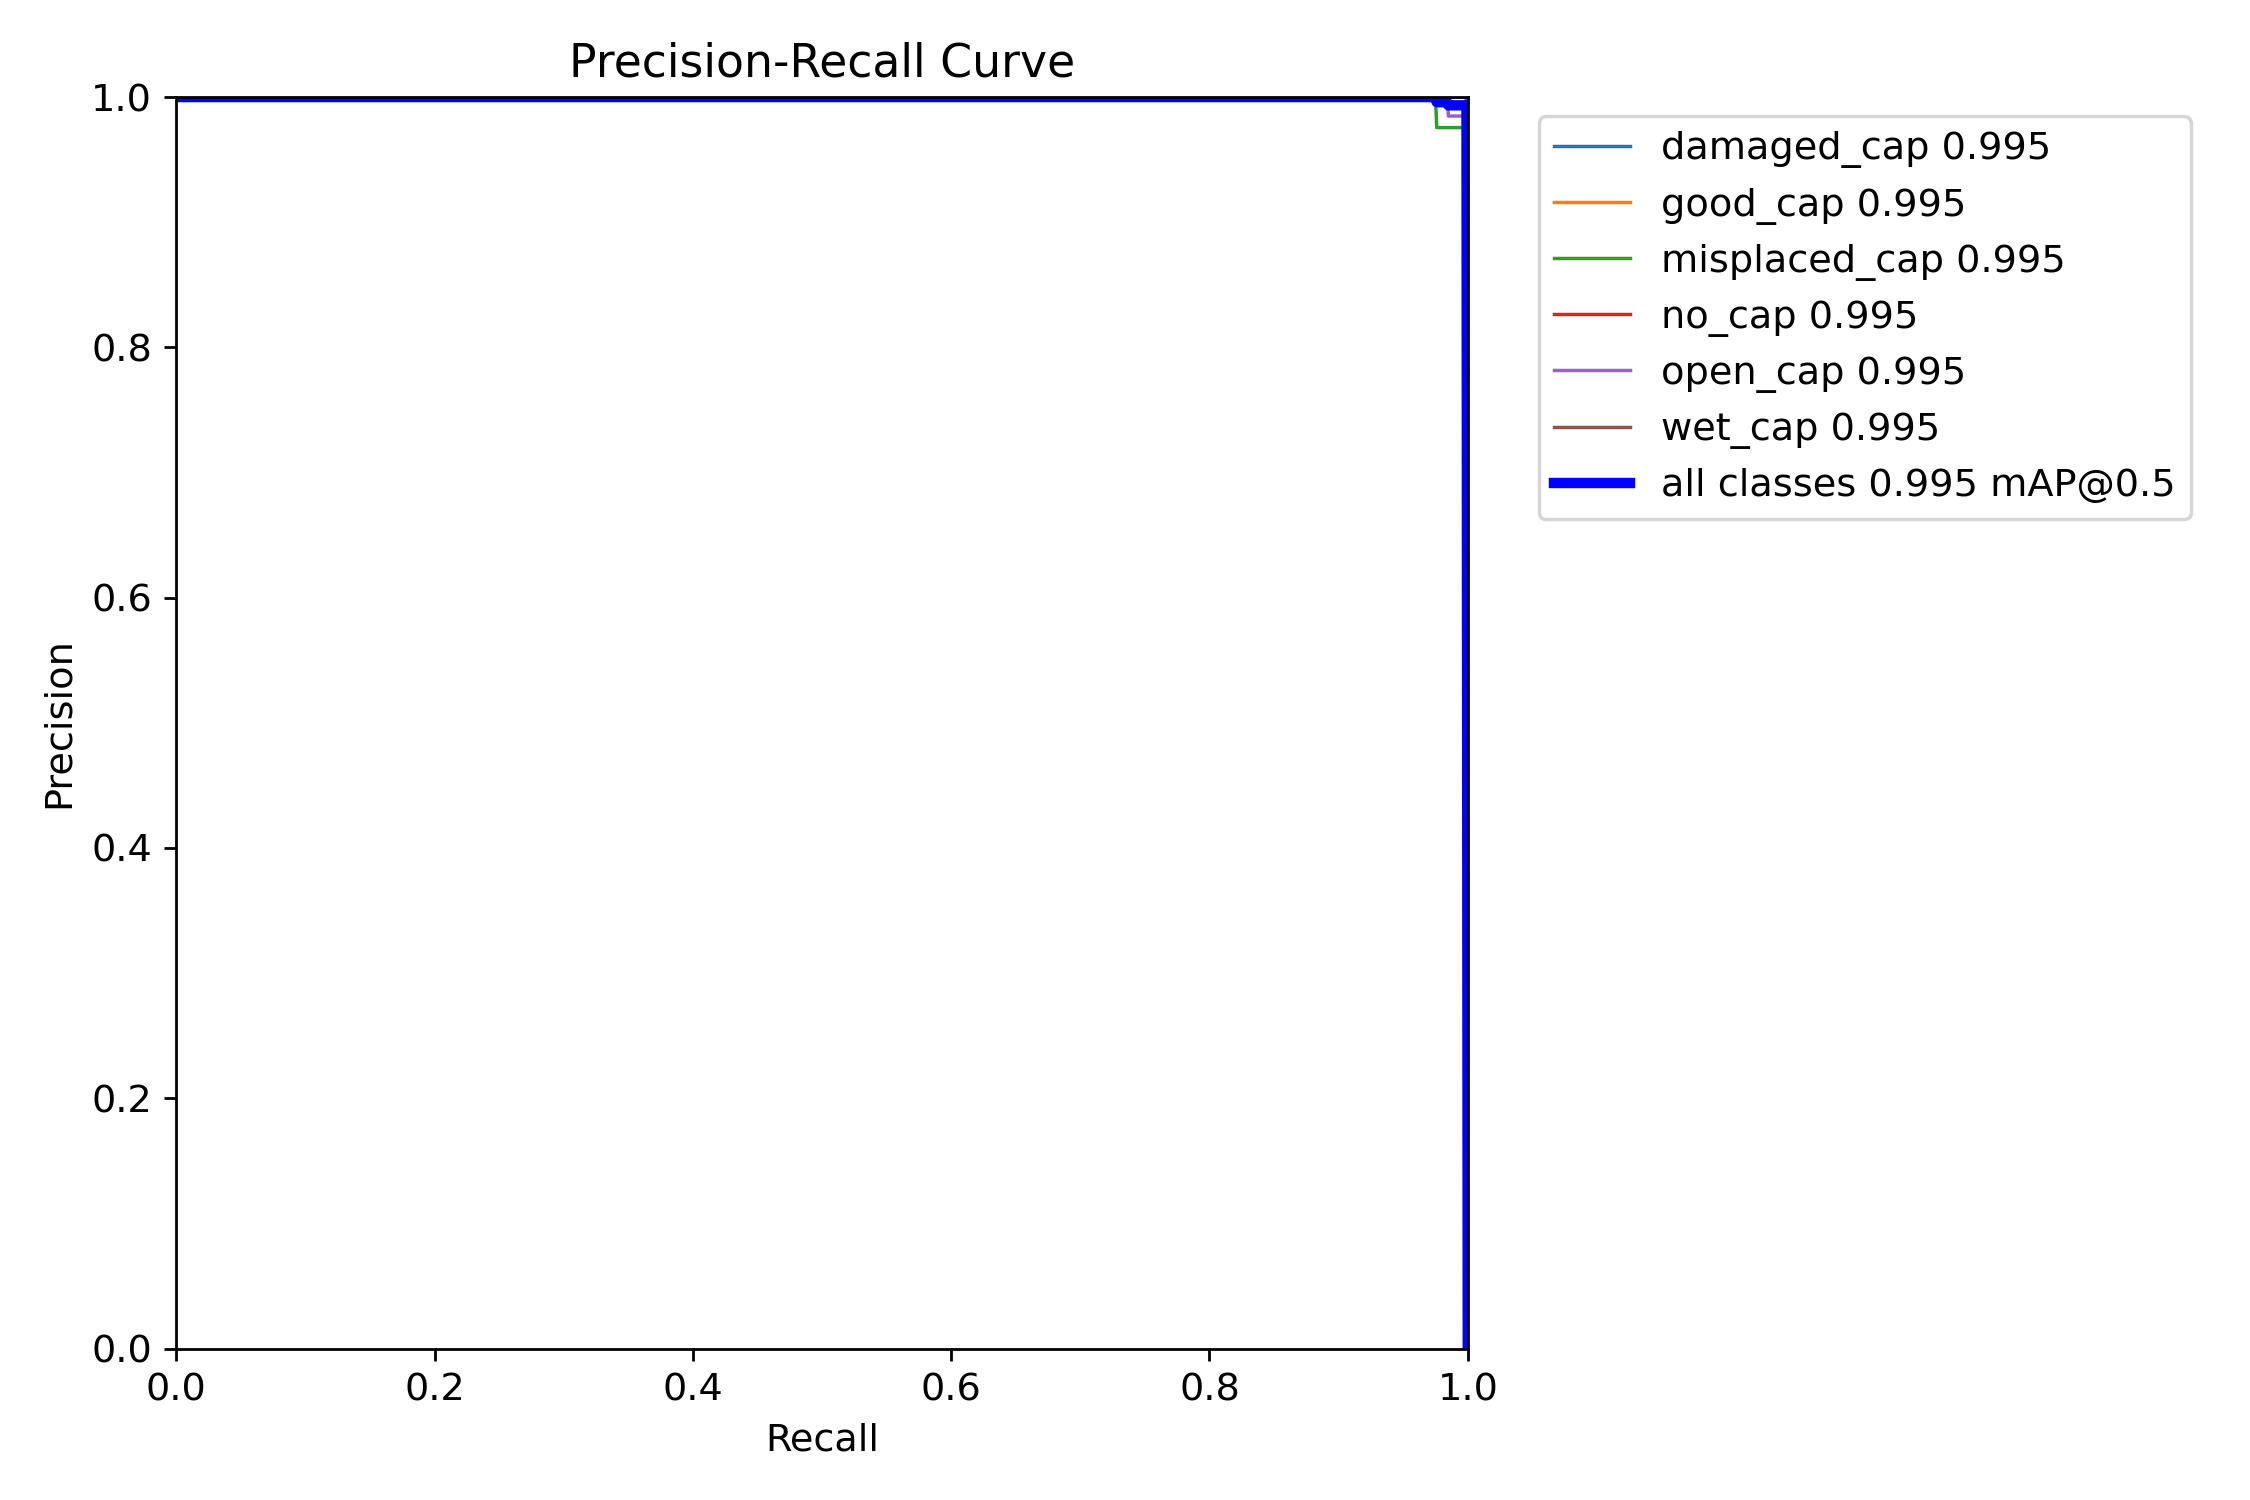
\includegraphics[width=0.49\textwidth]{figures/student_maskpr.png}\hfill
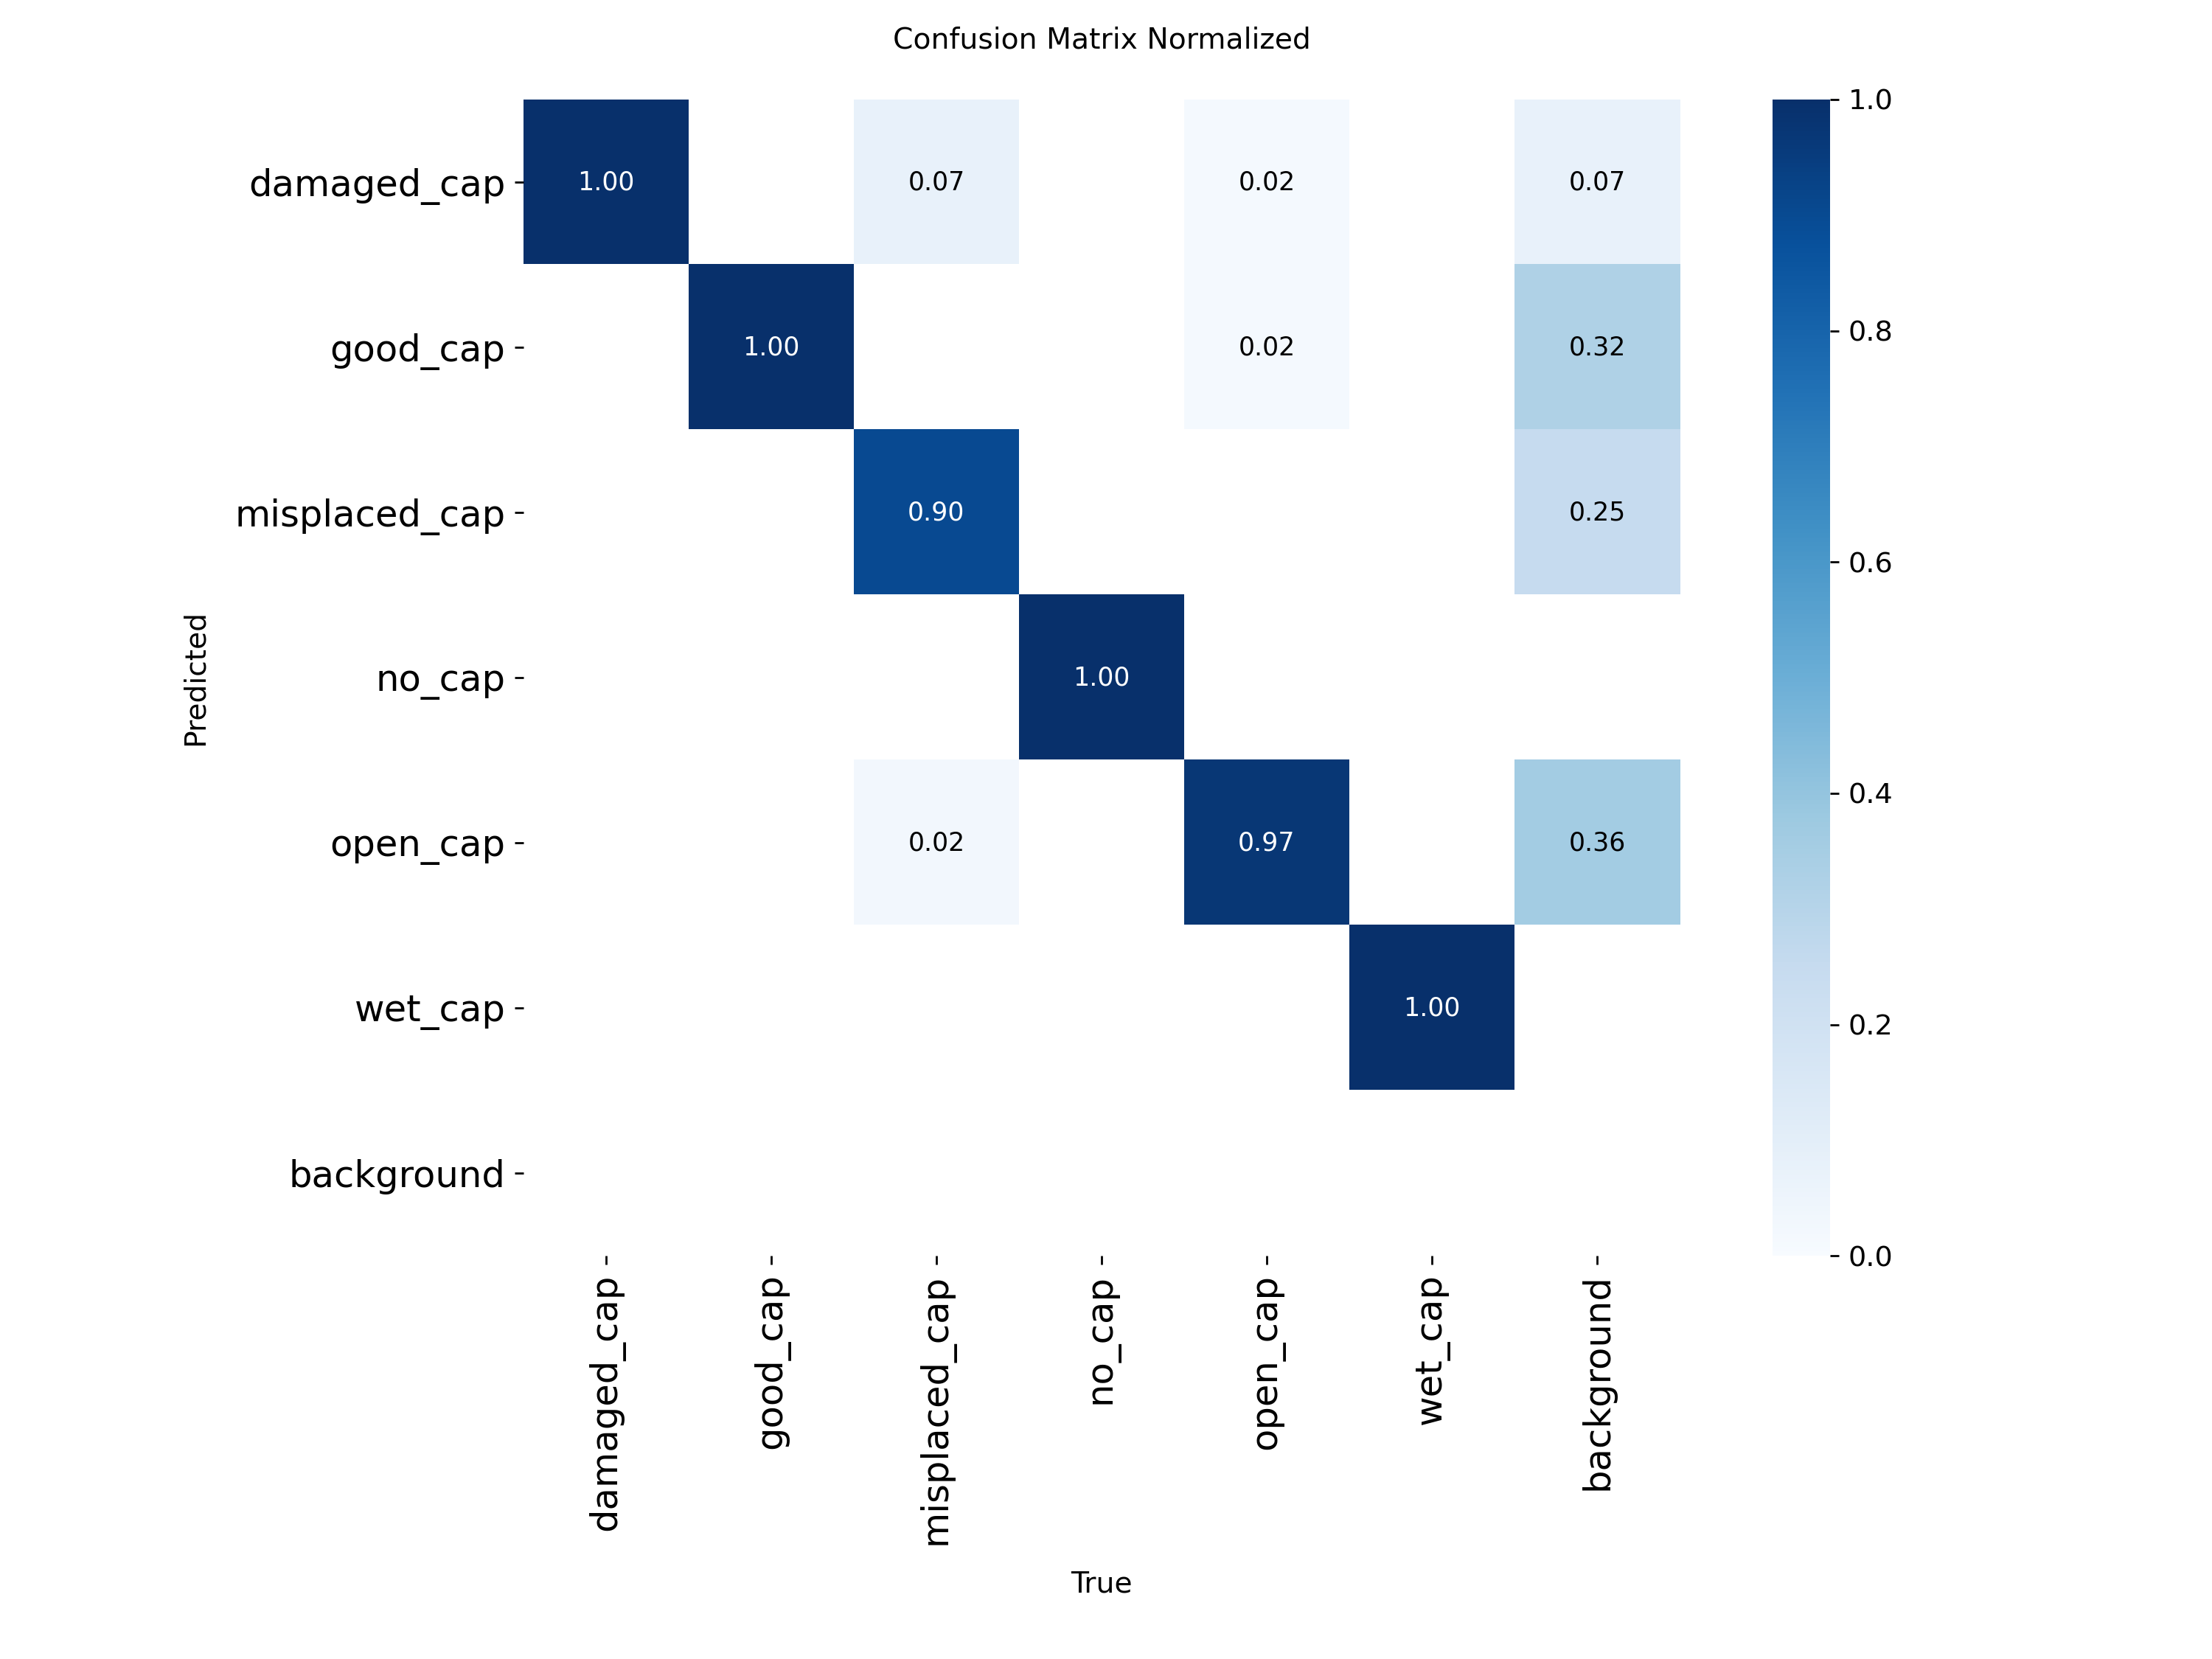
\includegraphics[width=0.49\textwidth]{figures/student_confusion.png}
\caption[Student precision--recall curves and confusion matrix]{Student YOLO11m-seg on the validation split: (left) mask precision--recall curves per class; (right) normalised confusion matrix.}
\label{fig:prcm}
\end{figure}

\subsection{Cap segmentation: trained versus deployed model}
\label{sec:res-seg}
Table~\ref{tab:seg} reports per-class segmentation metrics for the FP32 checkpoint and the deployed FP16 engine. Both reach AP@0.5 of 0.995 for every class. Converting to FP16 changes overall mAP@0.5:0.95 by at most 0.0013 and any single class by at most 0.006. The lowest strict-IoU score is for good-cap masks (0.893), where the boundary against the bottle neck is least distinct.

\begin{table}[htbp]
\centering
\caption{Station 1 segmentation on the held-out test split ($n=354$)}
\label{tab:seg}
\footnotesize
\begin{tabular}{|l|c|c|c|c|}
\hline
 & \multicolumn{2}{c|}{\textbf{FP32 PyTorch}} & \multicolumn{2}{c|}{\textbf{FP16 TensorRT}} \\ \hline
\textbf{Class (support)} & \textbf{Mask AP$_{50:95}$} & \textbf{Box AP$_{50:95}$} & \textbf{Mask} & \textbf{Box} \\ \hline
damaged (31) & 0.927 & 0.952 & 0.931 & 0.958 \\ \hline
good (201) & 0.893 & 0.904 & 0.894 & 0.903 \\ \hline
misplaced (15) & 0.941 & 0.930 & 0.942 & 0.930 \\ \hline
no cap (30) & 0.915 & 0.922 & 0.915 & 0.922 \\ \hline
open (38) & 0.935 & 0.928 & 0.933 & 0.929 \\ \hline
wet (39) & 0.953 & 0.929 & 0.953 & 0.930 \\ \hline
\textbf{All: mAP$_{50:95}$} & 0.927 & 0.927 & 0.928 & 0.929 \\ \hline
All: P / R & \multicolumn{2}{c|}{0.998 / 1.000} & \multicolumn{2}{c|}{0.998 / 1.000} \\ \hline
Valid: mAP$_{50:95}$ & 0.936 & 0.938 & 0.936 & 0.937 \\ \hline
\end{tabular}
\end{table}

Taking the highest-scoring detection above the 0.35 floor as the image label, top-1 classification is correct for 354 of 354 test images and 710 of 712 validation images (macro-F1 0.993, Cohen's $\kappa$ 0.996, MCC 0.996). Both validation errors are misplaced caps predicted as open caps; both are defect classes, so the bottle verdict is still \texttt{REJECT}.

\subsection{Product-level error and threshold analysis}
\label{sec:res-gate}
Table~\ref{tab:gate} replays the production gate image by image with the deployed engine. Each image counts as one bottle seen by one view, because the dataset has no synchronised triplets. No defective cap is passed and no good cap is rejected. With zero observed events, the exact Clopper--Pearson~\cite{clopper1934} 95\% upper bound on a rate with $n$ trials is $1-0.025^{1/n}$, which gives 2.4\% false accept and 1.8\% false reject on the test split.

\begin{table}[htbp]
\centering
\caption{Production gate replayed with the FP16 engine (defaults $\tau_p=0.75$, $\tau_d=0.45$, $\tau_u=0.40$)}
\label{tab:gate}
\footnotesize
\begin{tabular}{|l|c|c|}
\hline
 & \textbf{Valid} & \textbf{Test} \\ \hline
PASS / REJECT / UNCERTAIN / FAILED & 405 / 307 / 0 / 0 & 201 / 153 / 0 / 0 \\ \hline
False accept (defect $\rightarrow$ PASS) & 0/307 ($\leq1.2\%$) & 0/153 ($\leq2.4\%$) \\ \hline
False reject (good $\rightarrow$ REJECT) & 0/405 ($\leq0.9\%$) & 0/201 ($\leq1.8\%$) \\ \hline
Auto-decided accuracy & 1.000 & 1.000 \\ \hline
\multicolumn{3}{l}{\scriptsize Parentheses: Clopper--Pearson 95\% upper bound.}
\end{tabular}
\end{table}

We swept $\tau_p\in[0.50,0.95]$ and $\tau_d\in[0.25,0.65]$ (Figure~\ref{fig:sweep}). No false accept or false reject occurs at any grid point. The defect threshold has no effect over its whole range, because the engine emits no wrong-polarity score above 0.01 on either split: there is no defect score on good caps and no good-cap score on defective caps. The pass threshold controls only the review load. Good-cap top scores lie in $[0.856, 0.921]$ on test (median 0.897), so review routing starts between $\tau_p=0.85$ and $0.90$; at $0.90$, 34.5\% of test bottles and 36.0\% of validation bottles go to review. The default $\tau_p=0.75$ leaves a margin of $0.106$ below the lowest good-cap score. Defective caps score between 0.820 and 0.941 on test, 0.37 above $\tau_d$. Accuracy is identical across bounding-box-area terciles; the only validation errors fall in the largest tercile.

\begin{figure}[htbp]
\centering
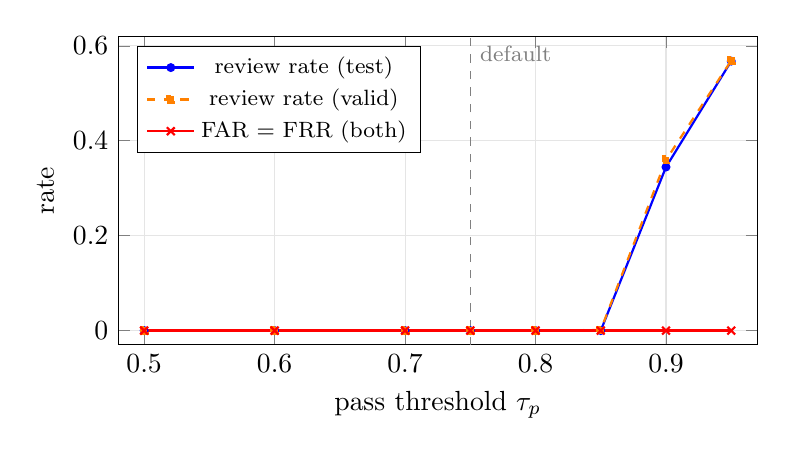
\begin{tikzpicture}
\begin{axis}[width=0.8\textwidth, height=5.5cm, xlabel={pass threshold $\tau_p$}, ylabel={rate}, ymin=-0.03, ymax=0.62, xmin=0.48, xmax=0.97, legend pos=north west, legend style={font=\footnotesize}, grid=major, grid style={gray!20}]
\addplot[blue, thick, mark=*, mark size=1.2pt] coordinates {(0.50,0) (0.60,0) (0.70,0) (0.75,0) (0.80,0) (0.85,0) (0.90,0.3446) (0.95,0.5678)};
\addplot[orange, thick, dashed, mark=square*, mark size=1.2pt] coordinates {(0.50,0) (0.60,0) (0.70,0) (0.75,0) (0.80,0) (0.85,0.0014) (0.90,0.3596) (0.95,0.5688)};
\addplot[red, thick, mark=x] coordinates {(0.50,0) (0.60,0) (0.70,0) (0.75,0) (0.80,0) (0.85,0) (0.90,0) (0.95,0)};
\draw[gray, dashed] (axis cs:0.75,-0.03) -- (axis cs:0.75,0.62) node[below right, font=\footnotesize]{default};
\legend{review rate (test), review rate (valid), FAR $=$ FRR (both)}
\end{axis}
\end{tikzpicture}
\caption[Gate threshold sweep]{Gate threshold sweep with the FP16 engine ($\tau_d=0.45$; every other $\tau_d$ in $[0.25,0.65]$ gives identical curves).}
\label{fig:sweep}
\end{figure}

\subsection{Fill-level estimation (O2)}
\label{sec:res-fill}
Table~\ref{tab:filldet} reports both Station 2 detectors on their held-out test splits at 640\,px. The meniscus detector localises the surface reliably at IoU 0.5 (AP 0.923) but loosely at strict IoU (AP@0.5:0.95 of 0.458). Because Eq.~\eqref{eq:rfill} uses only the box mid-line, this looseness affects the ratio far less than the strict-IoU score suggests. FP16 conversion leaves the meniscus detector unchanged but lowers the bottle detector's AP@0.5:0.95 from 0.578 to 0.481; the deployed bottle engine is built at 640\,px although the detector was trained at 512\,px, and building it at its training resolution is the planned remedy.

\begin{table}[htbp]
\centering
\caption{Station 2 detectors on held-out test splits (640\,px)}
\label{tab:filldet}
\footnotesize
\begin{tabular}{|l|l|c|c|c|c|}
\hline
\textbf{Model (class, boxes)} & \textbf{Runtime} & \textbf{P} & \textbf{R} & \textbf{AP$_{50}$} & \textbf{AP$_{50:95}$} \\ \hline
\multirow{2}{*}{YOLOv8s (bottle, 356)} & FP32 & 0.855 & 0.880 & 0.935 & 0.578 \\ \cline{2-6}
 & TRT FP16 & 0.823 & 0.890 & 0.907 & 0.481 \\ \hline
\multirow{2}{*}{YOLOv8n (surface, 76)} & FP32 & 0.904 & 0.867 & 0.923 & 0.458 \\ \cline{2-6}
 & TRT FP16 & 0.883 & 0.882 & 0.921 & 0.459 \\ \hline
\end{tabular}
\end{table}

To isolate the effect of meniscus localisation on the estimate, the deployed engines were run on the 41 surface-test images. For each image the ratio from the predicted surface was compared with the ratio from the annotated surface, using the same predicted bottle box. Table~\ref{tab:fillerr} gives the results. In 31 of 35 evaluable images the ratio differs by at most 0.02, the median difference is 1 pixel (0.002 in ratio), and the fill state agrees in 34 of 35 images. The single disagreement is an overfilled bottle (annotated ratio 0.902) that was passed as acceptable (0.708).

\begin{table}[htbp]
\centering
\caption{Fill-ratio error from meniscus localisation (41 test images, TRT FP16)}
\label{tab:fillerr}
\footnotesize
\begin{tabular}{|l|r|}
\hline
No bottle detected (multi-bottle rack frames) & 4 \\ \hline
Bottle found, no surface associated & 2 \\ \hline
Evaluated & 35 \\ \hline
Median $|\Delta R|$ / MAE / 90th percentile / max & 0.002 / 0.023 / 0.022 / 0.300 \\ \hline
$|\Delta R|\leq0.02$ / $\leq0.05$ & 88.6\% / 91.4\% \\ \hline
Fill-state agreement (under / acceptable / over) & 34/35 (97.1\%) \\ \hline
Gate verdicts PASS / REJECT / UNCERTAIN & 27 / 7 / 1 \\ \hline
\end{tabular}
\end{table}

The large errors share one failure mode: when the true surface sits high in the neck, the detector fires on a horizontal structure lower on the body, such as a moulded shoulder rib, a glare band, or the edge of a gripping hand. The two missed surfaces are a tinted bottle held in a hand and a nearly full bottle. All four frames with no bottle detection come from the multi-bottle rack video, which the single-bottle design does not support; they are reported as \texttt{INSPECTION\_FAILED} rather than guessed.

\subsection{Label-defect prototype (O4)}
\label{sec:res-label}

\paragraph{Localisation.} Template matching located all four regions in all 120 NSC scans (480 of 480), taking about 120\,ms per scan on the CPU. The overlap rule never fired, so no region was re-assigned. Localisation therefore needed no labelled boxes and no GPU.

\paragraph{Colour versus grayscale models.} The first EfficientAD models were trained on colour crops. On good crops they flagged large bright areas of the white label background, which produced many false alarms. Retraining on grayscale crops, replicated to three channels, made the models attend to print texture and intensity instead of colour. Table~\ref{tab:label-colour} compares the two for the crop-level evaluation.

\begin{table}[htbp]
\centering
\caption{Label prototype: colour versus grayscale EfficientAD-Medium, crop-level}
\label{tab:label-colour}
\footnotesize
\begin{tabular}{|l|r|r|c|c|c|c|}
\hline
 & & & \multicolumn{2}{c|}{\textbf{Colour}} & \multicolumn{2}{c|}{\textbf{Grayscale}} \\ \hline
\textbf{ROI} & \textbf{Good} & \textbf{Bad} & \textbf{Recall} & \textbf{FP} & \textbf{Recall} & \textbf{FP} \\ \hline
ROI\_1 (logo, name) & 74 & 33 & 79\% & 11 & 93.9\% & 6 \\ \hline
ROI\_2 (ingredients) & 77 & 14 & 86\% & 7 & 92.9\% & 6 \\ \hline
ROI\_3 (address, dates, barcode) & 78 & 31 & 74\% & 8 & 93.5\% & 13 \\ \hline
ROI\_4 (``3 Way Care'' graphic) & 77 & 26 & 46\% & high & 92.3\% & 56 \\ \hline
\end{tabular}
\end{table}

\paragraph{Final per-region results.} ROI\_4 kept a very high false-alarm count after the switch to grayscale, which pointed to noisy defect annotations rather than the architecture. Its defects were re-annotated, new crops were added, and the model was retrained for 300 epochs on 116 good and 60 defective crops. Table~\ref{tab:label-roi} gives the current per-region results. The protocols differ, and the table says so: ROI\_1--3 were evaluated on the available crop sets, whose good crops overlap the training data; ROI\_4 was evaluated on a 20\% split (seed 20261029) that was separated after training but not used for training the threshold, so it is a post-training holdout rather than a fully independent estimate.

\begin{table}[htbp]
\centering
\caption{Label prototype: grayscale EfficientAD-Medium per region}
\label{tab:label-roi}
\footnotesize
\begin{tabular}{|l|l|c|c|c|c|c|}
\hline
\textbf{ROI} & \textbf{Evaluation set} & \textbf{Acc.} & \textbf{Prec.} & \textbf{Recall} & \textbf{F1} & \textbf{TP/TN/FP/FN} \\ \hline
ROI\_1 & Crop set (74 good, 33 bad) & 92.5\% & 83.8\% & 93.9\% & 88.6\% & 31/68/6/2 \\ \hline
ROI\_2 & Crop set (77 good, 14 bad) & 92.3\% & 68.4\% & 92.9\% & 78.8\% & 13/71/6/1 \\ \hline
ROI\_3 & Crop set (78 good, 31 bad) & 86.2\% & 69.0\% & 93.5\% & 79.5\% & 29/65/13/2 \\ \hline
ROI\_4 old & Holdout (15 good, 5 bad) & 45.0\% & 28.6\% & 80.0\% & 42.1\% & 4/5/10/1 \\ \hline
\textbf{ROI\_4 new} & \textbf{Holdout (23 good, 12 bad)} & \textbf{74.3\%} & \textbf{57.9\%} & \textbf{91.7\%} & \textbf{71.0\%} & \textbf{11/15/8/1} \\ \hline
\end{tabular}
\end{table}

All four regions catch more than 91\% of defective crops, slightly below the 95\% recall that the threshold calibration targeted. Precision is the weak side: the models flag 6--13 of about 75 good crops in ROI\_1--3, and 8 of 23 good crops in ROI\_4.

\paragraph{Image-level status.} The image-level verdict (Eq.~\eqref{eq:labelrule}) has been tested only with provisional colour-mode thresholds fitted on 16 good and 16 defective scans that were also in the training data; a split-half check inside that subset caught 15 of 16 defective scans and flagged 3 of 16 good scans. Two earlier end-to-end runs illustrate why calibration matters: a run that loaded an outdated localiser caught only 21.4\% of defective scans, and a run with thresholds on the wrong score scale flagged all 120 scans (recall 1.0, accuracy 0.35). A full 120-scan run with the grayscale models and recalibrated thresholds, on held-out scans, has not yet been done.

\paragraph{Latency.} On a 16-core CPU the ONNX anomaly models take about 7\,s per crop, or about 25\,s per scan. During training the EfficientAD-Medium models ran at roughly 50\,ms per crop on the GPU, so GPU deployment is required before the prototype can approach line rate.

\section{Performance Evaluation}
\label{sec:performance-evaluation}

\subsection{Network latency (O3)}
Table~\ref{tab:latency} isolates the network from the rest of the pipeline. TensorRT FP16 reduces the three-view cap network time from 21.0\,ms (PyTorch FP32) to 7.4\,ms, a 2.8$\times$ speed-up, and the single-image fill detectors drop from 8.8 and 8.3\,ms to 1.3 and 1.1\,ms. ONNX Runtime on the CPU needs 510\,ms for the cap batch, which is too slow for the line. Measured end to end through the predictor, three 2048-pixel views take 20.1\,ms, of which about 13\,ms is host-side resizing and mask post-processing that grows with batch size and is not accelerated by the engine.

\begin{table}[htbp]
\centering
\caption{Per-call latency (ms, median of 100) inside the production container}
\label{tab:latency}
\footnotesize
\begin{tabular}{|l|l|r|r|r|}
\hline
\textbf{Model / input} & \textbf{Runtime} & \textbf{Network} & \textbf{Pre+post} & \textbf{Wall} \\ \hline
\multirow{3}{*}{Cap seg., 3 views $2048^2$} & PyTorch FP32 & 20.97 & 12.47 & 33.79 \\ \cline{2-5}
 & TRT FP16 & 7.44 & 12.35 & 20.12 \\ \cline{2-5}
 & ORT CPU FP32$^{*}$ & 509.89 & 16.68 & 526.43 \\ \hline
Cap seg., 3 views $640^2$ & TRT FP16 & 7.39 & 7.56 & 15.25 \\ \hline
Cap seg., 1 view $2048^2$ & TRT FP16 & 3.90 & 4.38 & 8.59 \\ \hline
\multirow{2}{*}{Bottle detector} & PyTorch FP32 & 8.77 & 2.11 & 11.21 \\ \cline{2-5}
 & TRT FP16 & 1.26 & 2.07 & 3.60 \\ \hline
\multirow{2}{*}{Meniscus detector} & PyTorch FP32 & 8.34 & 2.52 & 11.15 \\ \cline{2-5}
 & TRT FP16 & 1.13 & 2.33 & 3.76 \\ \hline
Fill engine (both detectors + Eq.~\eqref{eq:rfill}) & TRT FP16 & \multicolumn{3}{c|}{p50 7.34 / p95 10.23} \\ \hline
Fill gate (Alg.~\ref{alg:fillgate}) & CPU & \multicolumn{3}{c|}{p50 0.028 / p99 0.059} \\ \hline
\multicolumn{5}{l}{\scriptsize $^{*}$20 calls. Pre+post: Ultralytics pre-processing and post-processing.}
\end{tabular}
\end{table}

\subsection{Closed-loop stress test}
The Station 1 stress test drives the full production path inside the container for 500 cycles: TensorRT inference, extraction of mask polygons at native resolution, the gate, a synchronous SQLite (WAL) transaction that stores the three raw frames with labels, and overlay rendering. It cycles through the 354 test images, grouped three per bottle. Table~\ref{tab:stress} gives the breakdown. The median cycle is 299\,ms, or 163 bottles per minute unpaced. In a second run paced at 150 bottles per minute for 300 cycles, the line sustained 126.7 bottles per minute with a 99th-percentile cycle of 448\,ms; the JPEG decode of each 2048-pixel triplet falls outside the timed cycle, which is why the paced run fell short. No database write failed in either run.

\begin{table}[htbp]
\centering
\caption{Station 1 closed-loop stress test, 500 unpaced cycles (ms)}
\label{tab:stress}
\footnotesize
\begin{tabular}{|l|r|r|r|}
\hline
\textbf{Stage} & \textbf{p50} & \textbf{p95} & \textbf{p99} \\ \hline
Inference (3 views, incl.\ mask polygons) & 67.15 & 122.17 & 124.69 \\ \hline
Quality gate & 0.12 & 0.15 & 0.18 \\ \hline
SQLite WAL audit (3 raw frames) & 176.48 & 251.87 & 276.67 \\ \hline
Overlay rendering (3 views) & 41.59 & 43.21 & 43.91 \\ \hline
\textbf{Total closed-loop cycle} & \textbf{299.18} & \textbf{392.05} & \textbf{428.71} \\ \hline
\end{tabular}
\end{table}

The dominant cost is not the network. Storing three 2048-pixel frames synchronously takes 176\,ms, and most of the 67\,ms inference stage is mask-polygon extraction at native resolution. Station 2's service path (both engines, gate, audit, and overlay) takes 62.8\,ms at the median and 111.5\,ms at the 99th percentile over 500 frames, because it stores one frame instead of three.

\section{Validation}
\label{sec:validation}

Validation relied on hold-out sets at every level. The cap models were selected on the 712-image validation split and reported on the 354-image test split, which was not used for selection or threshold setting; agreement between the two splits (Table~\ref{tab:seg}) shows no sign of over-fitting to the selection set. Class-sensitive statistics were used because the classes are imbalanced: per-class AP, macro-F1 0.993, Cohen's $\kappa$ 0.996, and MCC 0.996 on validation, and exact binomial bounds wherever an error count is zero (Table~\ref{tab:gate}). The fill estimate was validated against annotated surfaces on a held-out split, isolating meniscus error from bottle-box error. During system integration the deployed cap engine was also run on photographs of our own bottles, which the model had never seen in training or evaluation, and its verdicts on these were satisfactory. For the label prototype, the strongest validation available is the ROI\_4 post-training holdout; the other regions still need an independently reserved test set.

\section{Comparative Analysis}
\label{sec:comparative-analysis}

\subsection{Why a segmentation detector replaced the Phase 1 classifier}
\label{sec:why-seg}
Phase 1 inspected caps in two stages: a YOLO detector found bottles and caps, and a MobileNetV3-Small classifier labelled the cap crop as good, defective, or missing. Before redesigning Station 1, five whole-image cap classifiers were benchmarked on a separate four-class dataset (7,540 images; 308-image test split). Table~\ref{tab:classifiers} gives the results.

\begin{table}[htbp]
\centering
\caption{Whole-image cap classifiers (separate 4-class dataset, $N_{\text{test}}=308$). GPU: PyTorch, batch 1; CPU: ONNX Runtime INT8}
\label{tab:classifiers}
\footnotesize
\begin{tabular}{|l|r|r|r|r|r|r|}
\hline
\textbf{Model} & \textbf{Acc.\ \%} & \textbf{mF1 \%} & \textbf{Damaged F1} & \textbf{Params (M)} & \textbf{GPU ms} & \textbf{CPU ms} \\ \hline
MobileNetV3-L~\cite{howard2019} & 96.43 & 94.75 & 0.857 & 4.21 & 9.36 & 4.77 \\ \hline
EfficientNetV2-S~\cite{tan2021} & 95.78 & 93.96 & 0.831 & 20.18 & 38.86 & 20.82 \\ \hline
ShuffleNetV2~\cite{ma2018} & 94.81 & 92.84 & 0.794 & 1.26 & 8.55 & 3.48 \\ \hline
ResNet-50~\cite{he2016} & 94.81 & 92.30 & 0.788 & 23.52 & 13.14 & 11.19 \\ \hline
DeiT-Tiny~\cite{touvron2021} & 94.81 & 92.69 & 0.788 & 5.53 & 12.64 & 7.07 \\ \hline
\end{tabular}
\end{table}

These numbers come from a different dataset and label set, so they are not directly comparable with Station 1. They informed the redesign in two ways. First, even the best classifier stayed below 0.86 F1 on damaged caps, the class whose evidence is finest. Second, a classifier returns no location, whereas the gate and the audit record need the cap's region (mask area, polygon, and per-view evidence). Table~\ref{tab:phase-compare} sets the two Station 1 designs side by side.

\begin{table}[htbp]
\centering
\caption{Phase 1 versus Phase 2 cap inspection (different datasets and label sets; indicative only)}
\label{tab:phase-compare}
\footnotesize
\begin{tabularx}{\textwidth}{|p{3.3cm}|X|X|}
\hline
 & \textbf{Phase 1: YOLO detector + MobileNetV3-Small} & \textbf{Phase 2: distilled YOLO11m-seg} \\ \hline
Classes & 3 (good, defective, missing) & 6 (good, damaged, misplaced, missing, open, wet) \\ \hline
Output & Class label per cap crop & Class, box, and mask per cap in one pass \\ \hline
Detector accuracy & P 0.869, R 0.973, mAP@0.5 0.958, mAP@0.5:0.95 0.786 & P 0.998, R 1.000, mAP@0.5 0.995, mask mAP@0.5:0.95 0.928 (FP16, test) \\ \hline
Cap classification & 86.5\% accuracy (P = R = 0.870) & 100\% top-1 on test (354/354); 99.7\% on validation \\ \hline
Product-level errors & Not measured & FAR 0/153, FRR 0/201 \\ \hline
Evaluation split & Final training epoch, validation & Untouched test split, FP32 and deployed FP16 \\ \hline
Latency & 466--678\,ms per uploaded image (dashboard, development machine) & 7.4\,ms network, 20.1\,ms predictor for three views \\ \hline
\end{tabularx}
\end{table}

\subsection{Comparison with the literature}
Direct numerical comparison with Table~\ref{tab:lit-compare} is not meaningful because every study uses a different product and dataset. Qualitatively, Phase 2 differs in what it reports: product-level false-accept and false-reject rates with exact bounds, as Ban\'us \textit{et al.}~\cite{banus2021} also do; a threshold sweep with an explicit margin, which none of the reviewed studies report; a measured fill ratio instead of a fill class~\cite{chatchapol2024}; and per-stage and closed-loop latency on the deployed system.

\section{Model Optimization \& Innovation}
\label{sec:model-optimization}

\paragraph{Optimisation steps and their effect.}
\begin{itemize}
    \item \textbf{Feature distillation:} 62.1\,M $\rightarrow$ 22.3\,M parameters (2.8$\times$), 297.4 $\rightarrow$ 113.0 GFLOPs, 19.0 $\rightarrow$ 7.8\,ms per image in FP32, with equal mAP@0.5 and +0.015 mask mAP@0.5:0.95 on test.
    \item \textbf{TensorRT FP16:} cap network 21.0 $\rightarrow$ 7.4\,ms for three views (2.8$\times$); fill detectors 8.8 $\rightarrow$ 1.3\,ms and 8.3 $\rightarrow$ 1.1\,ms; accuracy change $\leq0.0013$ mAP for the cap model.
    \item \textbf{Dynamic batching:} the three views share one execution instead of three.
    \item \textbf{Grayscale label crops:} recall on ROI\_1--3 raised from 74--86\% to 93--94\%.
\end{itemize}

\paragraph{Innovative aspects.} The contributions specific to this project are: (i) feature distillation at the three YOLO11 blocks that carry texture, multi-scale context, and attention, with $L_2$-normalised alignment that reduces to a cosine distance (Eq.~\eqref{eq:cosine}); (ii) an asymmetric multi-view gate whose thresholds are analysed for margin and review load; (iii) a closed-form fill ratio with a derived sensitivity and a confidence-gated review band; and (iv) a label prototype that combines training-free localisation with good-only anomaly models and counterfactual explanations.

\paragraph{Failed or abandoned attempts.} PatchCore was abandoned for the label task because its memory bank made inference too slow. A YOLO11m localiser with SAHI tiling was trained for the label regions but replaced by template matching, which is deterministic and needs no boxes. Colour-trained label models were replaced by grayscale ones. The first cap engine used a static batch of 1 and silently ran the three views sequentially until it was rebuilt with a dynamic profile. The deployed bottle engine at 640\,px loses 0.097 AP@0.5:0.95 against FP32; this is not yet fixed.

\section{Summary Against the Stated Targets}
\label{sec:targets}
Table~\ref{tab:targets} compares every measured quantity with its target, including the misses. The false-accept and false-reject limits follow from the recall ($\geq0.97$) and precision ($\geq0.93$) targets, and the 200\,ms cycle from a line rate of 300 bottles per minute.

\begin{table}[htbp]
\centering
\caption{All targets and outcomes (test split unless noted)}
\label{tab:targets}
\footnotesize
\begin{tabular}{|l|c|c|c|}
\hline
\textbf{Quantity} & \textbf{Target} & \textbf{Measured} & \textbf{Met} \\ \hline
Cap image-level accuracy & $\geq0.93$ & 1.000 & yes \\ \hline
Cap false accept / false reject & $\leq3\%$ / $\leq7\%$ & 0\% / 0\% & yes \\ \hline
Cap mask mAP@0.5:0.95 (FP16) & $\geq0.75$ & 0.928 & yes \\ \hline
Cap precision / recall (FP16) & $\geq0.93$ / $0.97$ & 0.998 / 1.000 & yes \\ \hline
Bottle det.\ AP@0.5 / 0.5:0.95 (FP16) & $\geq0.88$ / $0.75$ & 0.907 / 0.481 & yes / no \\ \hline
Meniscus P / R (FP16) & $\geq0.93$ / $0.97$ & 0.883 / 0.882 & no / no \\ \hline
Meniscus AP@0.5 / 0.5:0.95 (FP16) & $\geq0.88$ / $0.75$ & 0.921 / 0.459 & yes / no \\ \hline
Fill verdict agreement & $\geq0.93$ & 0.971 (34/35) & yes \\ \hline
GPU inference, 3 views (network) & $<100$\,ms & 7.4\,ms & yes \\ \hline
GPU inference stage, p95 & $<100$\,ms & 122\,ms & no \\ \hline
Closed-loop cycle, p50 (300 bottles/min) & $\leq200$\,ms & 299\,ms & no \\ \hline
Fill service cycle, p50 / p99 & $<100$\,ms & 62.8 / 111.5\,ms & p50 only \\ \hline
CPU inference (ORT, 3 views) & $<200$\,ms & 510\,ms & no \\ \hline
Label defect recall per ROI (crop level) & $\geq0.95$ & 0.917--0.939 & no \\ \hline
Label ROI\_4 precision (holdout) & --- & 0.579 & open \\ \hline
\end{tabular}
\end{table}

\section{Discussion and Limitations}
\label{sec:discussion}

\paragraph{Cap station.} The distilled student is accurate, stable under FP16, and well separated by its gate thresholds. The sweep also gives a monitoring rule for production: if the good-cap score distribution drifts down by more than about 0.1, for example under new lighting or bottle types, the default $\tau_p$ will begin routing good bottles to review before any defect is passed. The session-grouped held-out test identified under O1 is the next benchmark and will make results comparable across future model versions. A YOLO11m-seg trained without distillation would isolate the contribution of each distilled layer.

\paragraph{Fill station.} Measured against the annotated surface, the geometric rule is accurate wherever the meniscus is found; its errors are detection errors, not arithmetic errors. The rule assumes one upright bottle per frame and a visible meniscus inside the bottle box. The analysis isolates meniscus error only, because the surface dataset has no bottle annotations, so bottle-box error is bounded analytically (Eq.~\eqref{eq:prop}) rather than measured. No physical fill-volume ground truth was available.

\paragraph{Label prototype: unresolved ROI limitations.}
\begin{itemize}
    \item \textbf{False alarms.} ROI\_4 precision is 57.9\% on its holdout, and ROI\_3 flags 13 of 78 good crops; the line would discard good tubes at an unacceptable rate if deployed today.
    \item \textbf{Image-level labels.} Defective scans are labelled per image, not per region: only 14 of 42 defective scans have a defect in ROI\_2 and 26 in ROI\_4, which dilutes threshold calibration.
    \item \textbf{No independent test set.} Thresholds for ROI\_1--3 were fitted on data that overlaps training, and the image-level thresholds are provisional.
    \item \textbf{Controlled acquisition only.} All 120 scans are flat, evenly lit, unwrapped images. Specular reflections on the glossy tube, camera jitter, motion blur, and uncontrolled shop-floor lighting are not represented, and template matching with a fixed scale has not been tested under them; a change in scan resolution or label artwork requires new templates.
    \item \textbf{Latency.} About 25\,s per scan on the CPU; GPU deployment of the anomaly models is still to be done.
\end{itemize}

\paragraph{Throughput.} Real-time capability depends on the input/output around the network more than on the network. Writing the audit record asynchronously and down-sampling the stored frames would remove most of the 299\,ms cycle; neither is implemented in the measured system.
